\documentclass[a4paper,11pt]{jsarticle}

\usepackage{listings}
% 数式
\usepackage{amsmath,amsfonts}
\usepackage{bm}
% 画像
\usepackage[dvipdfmx]{graphicx}
\usepackage{here}
\usepackage{url}

\begin{document}

\title{知能情報実験II 5グループ\\設計書}
\author{195734B 知念直琉\\195723G 玉城賢勝\\195424F 佐藤幸大}
\date{\today}
\maketitle
\section{概要}
本プロジェクトでは以下の図\ref{play}のようなテトリスライクな落ち物パズルゲームを作成する。
本ゲームはシングルプレイであり、ゲームオーバーまでのスコアを競うゲームである。
点数によるランキングをリザルト画面に表示する。
\subsection{ゲームルール}
本パズルは基本7種類の落ち物があり、それらを横10マス、縦20マスで構成されたフィールドに落としていく。
ユーザから移動、回転の入力を命令を受け取り、それに応じて落ち物を動かして落としていく。
これらの落ち物を敷き詰めていき、横一列埋めることによって消すことができる。
列を消した時に点数が入る。また、一度にたくさんの列を消すほど得点が高くなる。一番上まで落ち物が積みあがり、落ち物の発生地点が埋まるとゲームオーバーとなる。

\section{仕様}
\subsection{画面構成}
以下の画面が存在する
\begin{enumerate}
\item メニュー画面
\item プレイ画面
\item ランキング画面
\end{enumerate}
\begin{figure}[H]
  \centering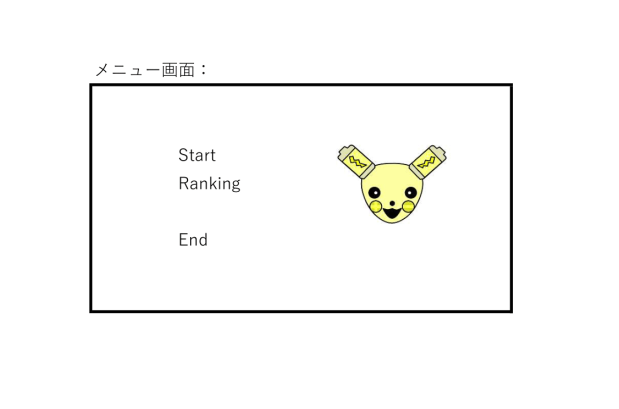
\includegraphics[clip,width=0.9\textwidth]{menu.png}
  \caption{メニュー画面}
  \label{menu}
\end{figure}
\begin{figure}[H]
  \centering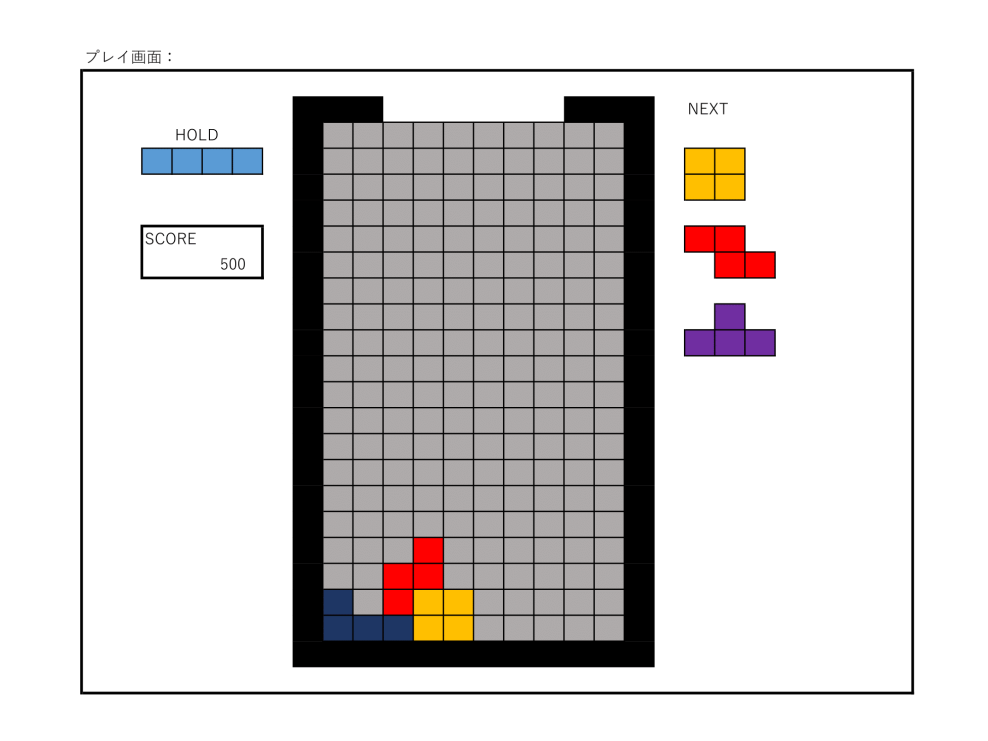
\includegraphics[clip,width=0.9\textwidth]{play.png}
  \caption{プレイ画面}
  \label{play}
\end{figure}
\begin{figure}[H]
  \centering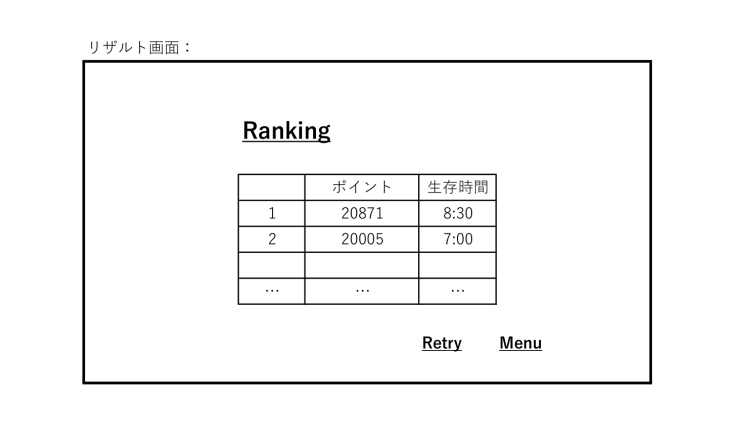
\includegraphics[clip,width=0.9\textwidth]{result.png}
  \caption{ランキング画面}
  \label{result}
\end{figure}

\subsubsection{画面遷移}
\begin{figure}[H]
  \centering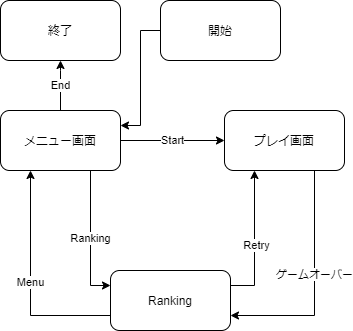
\includegraphics[clip,scale=0.5,width=1.0\textwidth]{tetorismo.png}
  \caption{画面遷移のフローチャート図}
  \label{tetoris}
\end{figure}
図\ref{tetoris}は画面遷移のフローチャート図である。
図\ref{menu}のゲームを始めたときに表示されるメニュー画面では,Startを押すと図\ref{play}のプレイ画面へ移動する.また,Rankingを押すと図\ref{result}のランキング画面へ移動することができ,Endを押すと,ゲームを終了する.\\
次に図\ref{play}のプレイ画面にてゲームオーバーになるとランキング画面へ移動する.\\
最後に図\ref{result}のランキング画面では,Retryを押すと,図\ref{play}のプレイ画面へ移動し,Menuを押すと,図\ref{menu}のメニュー画面へ移動する.

\subsection{テトリスのルール}
テトリスの基本ルールはWikipediaのテトリスのページ\cite{c0}に記載のルールを使用する。\par
本ゲームの仕様としては以下とする。
\begin{itemize}
  \item NEXTに表示されるミノの数は3つとする。
  \item HOLDを使用することができる。
  \item スコアは$10 \times 2^{一度に消した行数-1}$として計算する。
  \item ミノは60フレームで1ブロック分落下する。
  \item 5回行を消すとミノの落下するフレーム数を半分になる。\\(落下速度が倍になる)
\end{itemize}

\subsection{操作方法}
プレイ画面での操作方法は以下とする。
\begin{quote}
  \begin{description}
    \item[A] 左移動
    \item[D] 右移動
    \item[W] ハードドロップ(一番下までドロップ)
    \item[S] 落下速度をあげる
    \item[G] 左に回転する
    \item[H] 右に回転する
    \item[E] テトリミノをHOLD      
  \end{description}
\end{quote}

\section{詳細設計}
設計したクラス図の継承関係は以下の図\ref{classFigure}であり、has-a関係は図\ref{classFigure2}である。
\begin{figure}[H]
\begin{center}
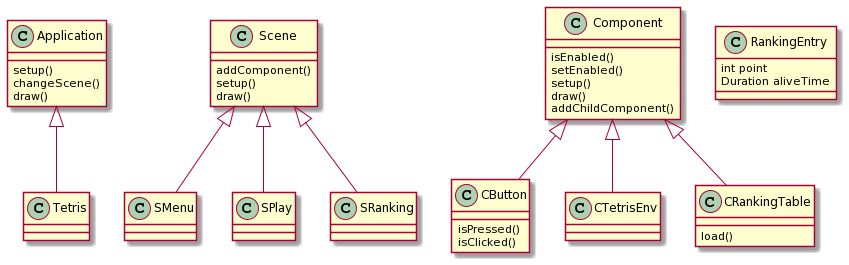
\includegraphics[width=\textwidth]{class.png}
\caption{クラス図の継承関係}
\label{classFigure}
\end{center}
\end{figure}

\begin{figure}[H]
\begin{center}
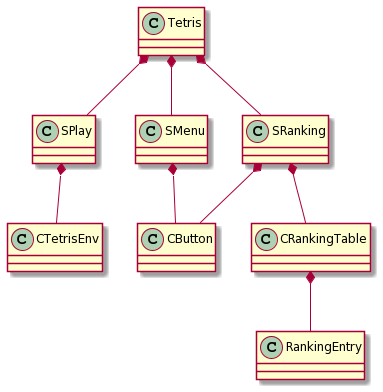
\includegraphics[width=0.6\textwidth]{class2.png}
\caption{クラス図のhas-a関係}
\label{classFigure2}
\end{center}
\end{figure}

図\ref{classFigure}の各クラスの概要を以下に示す。
\begin{description}
  \item[Application] アプリケーション毎に一つ。Sceneの管理等を行う。これを継承して具体的な実装を行う。
  \item[Scene] メニュー画面等、画面毎に一つ。構成部品であるComponentの配置、管理をここで行う。具体的なシーンはこれを継承して作成する。
  \item[Component] 構成部品。draw()を持ち、描画を行う。これを継承して具体的な実装を行う。  
  \item[Tetris] 大本のアプリケーションクラス
  \item[SMenu] メニュー画面の構成を行う
  \item[SPlay] ゲームをプレイ時の構成を行う
  \item[SRanking] ランキング画面時の構成を行う
  \item[CButton] ボタンを実装しているクラス。押されている間、クリックした瞬間を検知する。  
  \item[CTetrisEnv] テトリスのゲームのフィールド、スコア表示、Hold表示、next表示をまとめたコンポーネント。
  \item[CRankingTable] ランキングデータを読み込んで,ランキングのテーブルを表示するコンポーネント。
  \item[RankingEntry] ポイントと生存時間を格納するクラス。
  
\end{description}
\clearpage
CTetrisEnvコンポーネント内におけるゲームロジックのクラス図は以下の図\ref{logic}である。

本プレイ画面での実装では、CTetrisEnvはMVCデザインパターンにおけるView、TetrisCoreがModel、InputがControllの役割を担っている。

\begin{figure}[H]
\begin{center}
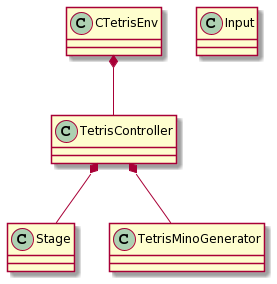
\includegraphics[width=75mm]{logic.png}
\caption{ゲームロジックのクラス図}
\label{logic}
\end{center}
\end{figure}

図\ref{logic}の各クラスの概要を以下に示す。
\begin{description}
\item[CTetrisEnv] ゲームロジックを包むコンポーネント
\item[TetrisCore] ゲームロジックの中枢を担い、ゲームの進行を行うクラス
\item[Stage] Stageのブロックの座標やミノの操作を行うクラス
\item[TetrisMinoGenerator] ミノの生成や次のミノの種類を返す
\item[Input] プレイヤーからの入力を受ける
\item[Mino] ミノの形のデータや回転の状態を持つクラス
\item[Coordinate] Stageにおける座標情報を持つクラス  
\end{description}

CTetrisEnvコンポーネント内におけるゲームロジックのシーケンス図は以下の図\ref{sequence}である。

\begin{figure}[htbp]
\begin{center}
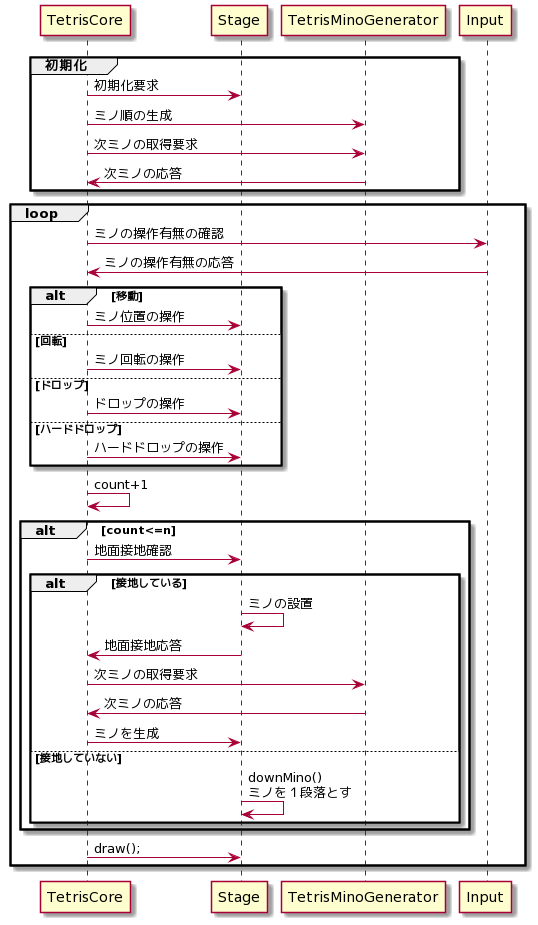
\includegraphics[width=0.8\textwidth]{sequence.png}
\caption{CTetrisEnv下のシーケンス図}
\label{sequence}
\end{center}
\end{figure}
\clearpage

\section{役割分担}
\begin{itemize}
  \item 設計等は基本的に全員で集まって行った
  \item メニュー画面の実装を佐藤が担当した。
  \item ランキング画面の実装を玉城が担当した。
  \item プレイ画面のリード実装を知念が担当した。
  \item プレイ画面のmodel部分の実装を知念が担当した。
  \item プレイ画面のview部分の実装を玉城が担当した。
\end{itemize}
作業時間は以下のようになった。
\begin{quote}
\begin{description}
\item[玉城] 約16時間
\item[佐藤] 約13時間
\item[知念] 約14時間
\end{description}
\end{quote}

\begin{thebibliography}{99}
  \bibitem{c0} テトリス-Wikipedia,\url{https://ja.wikipedia.org/wiki/%E3%83%86%E3%83%88%E3%83%AA%E3%82%B9},2020/11/07 参照.
\end{thebibliography}

\end{document}